\immediate\write18{makeindex C-1.nlo -s nomencl.ist -o C-1.nls}
\documentclass[12pt,a4paper]{report}
\usepackage[utf8]{inputenc}
\usepackage{vietnam}
\usepackage[left=3cm, right=2.2cm, top=2.5cm, bottom=2.5cm]{geometry}
\usepackage{amsmath}
\usepackage{float}
\usepackage{amssymb} 
\usepackage{graphicx} 
\usepackage[hidelinks, unicode]{hyperref}
\usepackage[labelsep=period]{caption}
\usepackage[table]{xcolor}
\usepackage{titletoc}
\usepackage{etoc}
\usepackage{mathptmx}
\usepackage{sectsty}
\usepackage{multirow}
\usepackage{booktabs, tabularx}
\usepackage{courier}
\usepackage{subfig}
\usepackage{nomencl}
\usepackage{titlesec}
\usepackage{enumitem}
\usepackage{anyfontsize}
\usepackage[fontsize=13pt]{scrextend}
\newcommand{\code}[1]{\texttt{#1}}
\renewcommand{\baselinestretch}{1.5}
\renewcommand{\nomname}{Danh mục ký hiệu và viết tắt}


\makenomenclature
\makeatletter
\titlecontents{chapter}[3cm] % <-- seems to set some specific left margin
{\color{black}\bfseries\addvspace{3mm}}
{\makebox[0cm][r]{\MakeUppercase\@chapapp\hspace{.5em}\thecontentslabel\hspace{0.75cm}}}
{} %     ^^^ pretendously zero width box puts its contents in the left margin
{\hfill\makebox[-2cm]{\thecontentspage}}  % 3cm = twice 1.5cm
\chapternumberfont{\Large}
\chaptertitlefont{\Large}

\titleformat{\chapter}[hang] 
{\normalfont\fontsize{14}{15}\bfseries}{CHƯƠNG \thechapter.}{1em}{} 
\titlespacing*{\chapter}{0pt}{-7pt}{7pt}

\titleformat{\section}
{\normalfont\fontsize{13}{15}\bfseries}{\thesection.}{1em}{}
\titlespacing*{\section}{0pt}{-5pt}{-6pt}  

\titleformat{\subsection}
{\normalfont\fontsize{13}{15}\bfseries\itshape}{\thesubsection.}{1em}{}
\titlespacing*{\subsection}{0pt}{-20pt}{-6pt}

\titleformat{\subsubsection}
{\normalfont\fontsize{13}{15}\itshape}{\thesubsubsection.}{1em}{}
\titlespacing*{\subsubsection}{0pt}{-20pt}{-6pt}


\newcommand{\subsubsubsection}[1]{\paragraph{#1}\mbox{}\\}


\setlist[itemize]{itemsep=-0.3em, topsep=0pt}
\setlength\parindent{0pt}
\setlength{\parskip}{10pt}
\setcounter{secnumdepth}{4}
\setcounter{tocdepth}{4}
\geometry{letterpaper}

% \title{\textbf{ĐỒ ÁN CÔNG NGHỆ MỎ}}
% \author{Bùi Trọng Nghĩa\\Diệp Công Trứ}

\begin{document}
\pagenumbering{gobble}
% \thispagestyle{empty}
\clearpage

\pdfbookmark{\contentsname}{content}
% \maketitle

\tableofcontents
\addcontentsline{toc}{section}{MỤC LỤC}

\listoffigures
\addcontentsline{toc}{section}{DANH SÁCH HÌNH VẼ}

\listoftables
\addcontentsline{toc}{section}{DANH SÁCH BẢNG BIỂU}

\printnomenclature
\addcontentsline{toc}{section}{DANH MỤC KÝ HIỆU VÀ VIẾT TẮT}

\clearpage
\pagenumbering{arabic}
\newpage

\chapter{CƠ SỞ LÝ THUYẾT}
\section{Các đặc tính dự báo}

\section{Phương pháp dự báo bằng mạng neuron nhân tạo}

\section{Các phương pháp khai thác nhân tạo}
Thông thường, trong giai đoạn đầu của một giếng khai thác dòng lưu chất từ vỉa sẽ khai thác nhờ áp suất vỉa (nếu áp suất vỉa lớn hơn tổng áp suất mất mát của hệ thống khai thác), giai đoạn này được gọi là khai thác tự phun. Nếu như áp suất vỉa không còn đủ lớn để có thể thắng được áp suất mất mát, dòng chảy trong giếng sẽ ``chết'' và giếng không thể tiếp tục khai thác tự phun được nữa. Hai nguyên nhân chính dẫn đến dòng trong giếng bắt đầu ``chết'' chính là:
	\begin{itemize}
		\item Áp suất dòng vào ở đáy giếng giảm xuống thấp hơn tổng áp suất mất mát của giếng,
		\item Tổng áp suất mất mát của giếng lớn hơn áp suất đáy giếng nhỏ nhất để có thể đưa được dòng lưu chất lên bề mặt.
	\end{itemize}
Trường hợp đầu tiên xảy ra khi lưu chất được khai thác khỏi vỉa sẽ dẫn tới áp suất của vỉa suy giảm theo thời gian cho tới khi không còn đủ lớn để thắng được áp suất mất mát của hệ thống khai thác. Đối với trường hợp thứ hai, thường do tăng mức độ cản trở dòng chảy trong hệ thống, có hai nguyên nhân dẫn đến điều này:
	\begin{itemize}
		\item Tỉ trọng của dòng lưu chất tăng do lượng khí đồng hành giảm,
		\item Các vấn đề cơ học như kích thước tubing nhỏ, lắng đọng cặn ...
	\end{itemize}
Khai thác nhân tạo được thực hiện khi dòng chảy trong giếng bắt đầu ``chết'' hoặc tăng lưu lượng khai thác của giếng. Hai phương pháp phổ biến nhất thường được lựa chọn để thực hiện khai thác nhân tạo là bơm điện li tâm chìm (ESP)\nomenclature{ESP}{Electrical Submersible Pump}; một máy bơm sẽ được đặt xuống lòng giếng dưới mực lưu chất trong giếng, bơm tăng áp suất để thắng được tổn thất áp suất trong hệ thống; và bơm ép khí từ bề mặt vào trong tubing khai thác để dòng lưu chất dễ dàng phun lên bề mặt hơn (gas lift). Ngoài ra vẫn còn một số phương pháp khai thác nhân tạo khác nhưng không được sử dụng phổ biến.\\

\subsection{Bơm điện li tâm chìm}
\subsubsection{Ứng dụng}
Được đưa vào ứng dụng trong thực tiễn từ năm 1920 tại mỏ Oklahoma, ESP có thể nâng lưu lượng khai thác thêm tới 1000 thùng trên ngày, gấp khoảng 2 đến 3 lần bơm cần (rod pump).

Ngày nay, bơm điện li tâm chìm thường được ứng dụng trong bơm ép nước (trên bờ), khai thác trên biển hoặc trong những trường hợp có sẵn nguồn điện và khai thác với lưu lượng lớn. ESP có thể được lắp đặt ở độ sâu 1,000 ft đến 10,000 ft đồng thời tăng lưu lượng khai thác thêm từ 200 bbl/d đến 20,000 bbl/d (Hình \ref{fig:rate-vs-depth}). Kỉ lục độ sâu và lưu lượng có thể sử dụng ESP là 15,000 ft và 30,000 bbl/d.\\

	\begin{figure}[h]
		\centering
		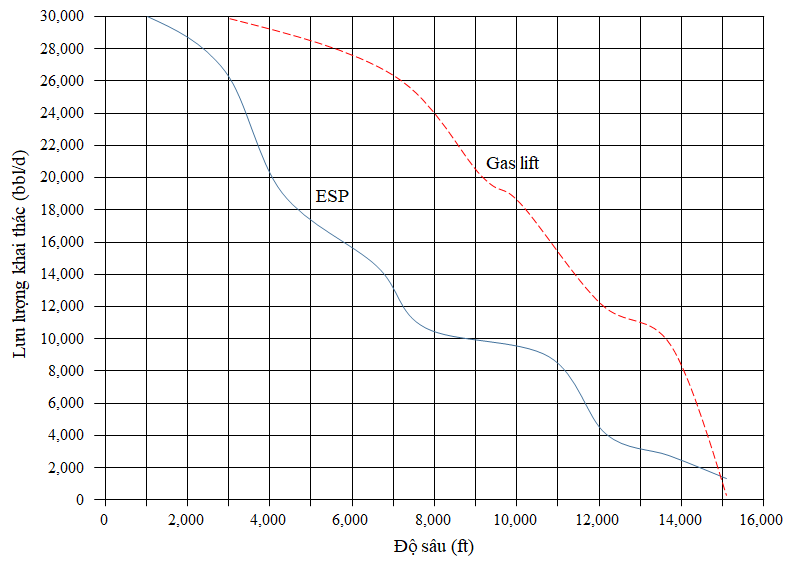
\includegraphics[scale=0.6]{fig/rate-vs-depth.png}
		\caption{Lưu lượng khai thác tối đa theo độ sâu}
		\label{fig:rate-vs-depth}
	\end{figure}

\subsubsection{Ưu điểm và hạn chế}

Một vài ưu điểm của bơm điện li tâm chìm có thể kể đến như sau:
	\begin{itemize}
		\item Thích hợp với khai thác lưu lượng lớn,
		\item Hiệu suất cao,
		\item Sử dụng tốt trong giếng khoan định hướng,
		\item Có thể sử dụng trong điều kiện khu dân cư,
		\item Thích hợp với hoạt động khai thác trên biển,
		\item Dễ dàng sử lý ăn mòn và lắng đọng.
	\end{itemize}
ESP cũng có một vài hạn chế:
	\begin{itemize}
		\item Phụ thuộc vào nguồn cung cấp năng lượng,
		\item Cần được vận hành trong điều kiện ổn định,
		\item Dễ bị ảnh hưởng bởi cát hay các vật chất gây ăn mòn,
		\item Quá trình sửa chửa khó khăn,
		\item Bị hạn chế trong vùng có nhiệt độ cao,
		\item Hiệu suất thấp đối với dầu có độ nhớt cao,
		\item Chi phí lắp đặt cao.\\
	\end{itemize}

\subsection{Gas lift}
Gas lift là phương pháp bơm ép khí vào cột lưu chất trong giếng để lưu chất có thể dễ dàng được khai thác hơn. Hầu hết khí được sử dụng trong bơm ép là khí tự nhiên có đặc tính trơ, được bơm ép vào trong tubing tại những vị trí đã được thiết kế trước, dựa trên ba nguyên lý chủ yếu: giảm tỉ trọng hỗn hợp lưu chất, năng lượng giản nở của khí và thay thế vị trí. Từ đó dòng lưu chất tại đáy giếng có thể tiếp tục được đưa lên bề mặt và giếng bắt đầu được khai thác trở lại hoặc nâng cao năng suất khai thác. Có thể chia gas lift thành hai loại là gas lift định kì và gas lift liên tục.

Đối với gas lift liên tục, dòng khí được bơm liên tục có kiểm soát vào trong tubing trong khi gas lift định kì sẽ thực hiện bơm khí theo chu kì nhất định khi lưu chất trong tubing có xu hướng tích tụ về đáy giếng. Sơ đồ một giếng khai thác sử dụng gas lift được thể hiện như sau:

	\begin{figure}[h]
		\centering
		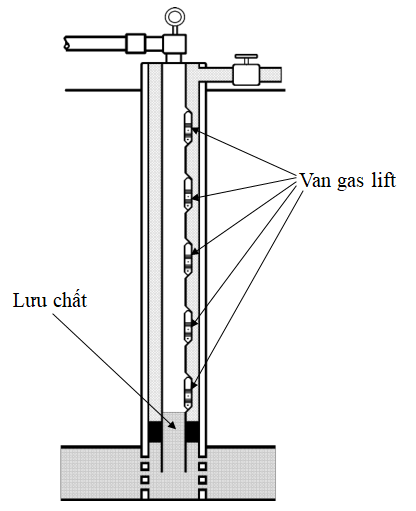
\includegraphics[scale=0.7]{fig/continuous-gas-lift.png}
		\caption{Sơ đồ giếng khai thác với gas lift}
		\label{fig:continuous-gas-lift}
	\end{figure}

Trong đó, đối với gas lift liên tục van thấp nhất sẽ được mở liên tục để thực hiện bơm ép khí, các van còn lại được vận hành tùy vào mục đích của người vận hành. Đối với gas lift định kì, các van sẽ được mở tùy theo thời gian bơm ép định kì đã lên theo kế hoạch và đóng trong những khoảng thời gian khác. Thông thường trong thời gian bơm ép van số 5 (theo sơ đồ Hình \ref{fig:continuous-gas-lift}) sẽ được mở trước tiên, các van khác được vận hành tùy theo mục đích.

Lưu lượng khí bơm ép cho mỗi giếng được phân chia tùy thuộc vào đặc tính của giếng đó. Trong phạm vi của luận án, tác giả sẽ đi vào xây dựng mô hình phân phối lưu lượng khí cho từng giếng theo cụm giếng chung hệ thống ống góp (manifold). Mô hình sẽ không phân biệt phương pháp gas lift liên tục hay định kì, chỉ đưa ra lưu lượng khí bơm ép cho mỗi giếng dưới điều kiện tổng lượng khí bơm ép xác định để đạt được lưu lượng dầu tối đa trong điều kiện bình tách có thể chịu được.\\

\subsubsection{Ứng dụng}
Lần đầu tiên gas lift được đưa vào trong khai thác năm 1846 tại Mĩ, tuy nhiên để sử dụng khai thác nước là chủ yếu. Đến năm 1930 gas lift mới thực sự được đưa vào ứng dụng trong ngành công nghiệp dầu khí cùng với sự ra đời của các mẫu van gas lift khác nhau. Vào những năm này gas lift được sử dụng do hai nguyên chính:
	\begin{itemize}
		\item Tăng mạnh lưu lượng khai thác trong khi năng lượng vỉa bắt đầu suy kiệt,
		\item Đem lại nhiều lợi ích kinh tế khi lượng khí bơm ép sau sử dụng có thể được tách và sử dụng lại, ít bị thất thoát trong quá trình sử dụng.
	\end{itemize}
Trong ngành công nghiệp dầu khí hiện đại, gas lift có những ứng dụng chính như sau:
	\begin{itemize}
		\item Đưa giếng trở lại khai thác sau khi đã kết thúc giai đoạn khai thác tự nhiên,
		\item Tăng lưu lượng khai thác,
		\item Loại bỏ thành phần lỏng trong các giếng khai thác khí,
		\item Xử lý những giếng lắng đọng cát trong giai đoạn bắn mở vỉa,
		\item Khai thác nước cho quá trình bơm ép nước.\\
	\end{itemize}

\subsubsection{Ưu điểm và hạn chế}


\section{Đường cong đặc tính gas lift}

\section{Giải thuật di truyền}
\subsection{Nguyên lý giải thuật}

\subsection{Bài toán tối ưu}

\section{Thuật toán}

\end{document}